% Options for packages loaded elsewhere
\PassOptionsToPackage{unicode}{hyperref}
\PassOptionsToPackage{hyphens}{url}
%
\documentclass[
]{article}
\usepackage{amsmath,amssymb}
\usepackage{iftex}
\ifPDFTeX
  \usepackage[T1]{fontenc}
  \usepackage[utf8]{inputenc}
  \usepackage{textcomp} % provide euro and other symbols
\else % if luatex or xetex
  \usepackage{unicode-math} % this also loads fontspec
  \defaultfontfeatures{Scale=MatchLowercase}
  \defaultfontfeatures[\rmfamily]{Ligatures=TeX,Scale=1}
\fi
\usepackage{lmodern}
\ifPDFTeX\else
  % xetex/luatex font selection
\fi
% Use upquote if available, for straight quotes in verbatim environments
\IfFileExists{upquote.sty}{\usepackage{upquote}}{}
\IfFileExists{microtype.sty}{% use microtype if available
  \usepackage[]{microtype}
  \UseMicrotypeSet[protrusion]{basicmath} % disable protrusion for tt fonts
}{}
\makeatletter
\@ifundefined{KOMAClassName}{% if non-KOMA class
  \IfFileExists{parskip.sty}{%
    \usepackage{parskip}
  }{% else
    \setlength{\parindent}{0pt}
    \setlength{\parskip}{6pt plus 2pt minus 1pt}}
}{% if KOMA class
  \KOMAoptions{parskip=half}}
\makeatother
\usepackage{xcolor}
\usepackage[margin=1in]{geometry}
\usepackage{color}
\usepackage{fancyvrb}
\newcommand{\VerbBar}{|}
\newcommand{\VERB}{\Verb[commandchars=\\\{\}]}
\DefineVerbatimEnvironment{Highlighting}{Verbatim}{commandchars=\\\{\}}
% Add ',fontsize=\small' for more characters per line
\usepackage{framed}
\definecolor{shadecolor}{RGB}{248,248,248}
\newenvironment{Shaded}{\begin{snugshade}}{\end{snugshade}}
\newcommand{\AlertTok}[1]{\textcolor[rgb]{0.94,0.16,0.16}{#1}}
\newcommand{\AnnotationTok}[1]{\textcolor[rgb]{0.56,0.35,0.01}{\textbf{\textit{#1}}}}
\newcommand{\AttributeTok}[1]{\textcolor[rgb]{0.13,0.29,0.53}{#1}}
\newcommand{\BaseNTok}[1]{\textcolor[rgb]{0.00,0.00,0.81}{#1}}
\newcommand{\BuiltInTok}[1]{#1}
\newcommand{\CharTok}[1]{\textcolor[rgb]{0.31,0.60,0.02}{#1}}
\newcommand{\CommentTok}[1]{\textcolor[rgb]{0.56,0.35,0.01}{\textit{#1}}}
\newcommand{\CommentVarTok}[1]{\textcolor[rgb]{0.56,0.35,0.01}{\textbf{\textit{#1}}}}
\newcommand{\ConstantTok}[1]{\textcolor[rgb]{0.56,0.35,0.01}{#1}}
\newcommand{\ControlFlowTok}[1]{\textcolor[rgb]{0.13,0.29,0.53}{\textbf{#1}}}
\newcommand{\DataTypeTok}[1]{\textcolor[rgb]{0.13,0.29,0.53}{#1}}
\newcommand{\DecValTok}[1]{\textcolor[rgb]{0.00,0.00,0.81}{#1}}
\newcommand{\DocumentationTok}[1]{\textcolor[rgb]{0.56,0.35,0.01}{\textbf{\textit{#1}}}}
\newcommand{\ErrorTok}[1]{\textcolor[rgb]{0.64,0.00,0.00}{\textbf{#1}}}
\newcommand{\ExtensionTok}[1]{#1}
\newcommand{\FloatTok}[1]{\textcolor[rgb]{0.00,0.00,0.81}{#1}}
\newcommand{\FunctionTok}[1]{\textcolor[rgb]{0.13,0.29,0.53}{\textbf{#1}}}
\newcommand{\ImportTok}[1]{#1}
\newcommand{\InformationTok}[1]{\textcolor[rgb]{0.56,0.35,0.01}{\textbf{\textit{#1}}}}
\newcommand{\KeywordTok}[1]{\textcolor[rgb]{0.13,0.29,0.53}{\textbf{#1}}}
\newcommand{\NormalTok}[1]{#1}
\newcommand{\OperatorTok}[1]{\textcolor[rgb]{0.81,0.36,0.00}{\textbf{#1}}}
\newcommand{\OtherTok}[1]{\textcolor[rgb]{0.56,0.35,0.01}{#1}}
\newcommand{\PreprocessorTok}[1]{\textcolor[rgb]{0.56,0.35,0.01}{\textit{#1}}}
\newcommand{\RegionMarkerTok}[1]{#1}
\newcommand{\SpecialCharTok}[1]{\textcolor[rgb]{0.81,0.36,0.00}{\textbf{#1}}}
\newcommand{\SpecialStringTok}[1]{\textcolor[rgb]{0.31,0.60,0.02}{#1}}
\newcommand{\StringTok}[1]{\textcolor[rgb]{0.31,0.60,0.02}{#1}}
\newcommand{\VariableTok}[1]{\textcolor[rgb]{0.00,0.00,0.00}{#1}}
\newcommand{\VerbatimStringTok}[1]{\textcolor[rgb]{0.31,0.60,0.02}{#1}}
\newcommand{\WarningTok}[1]{\textcolor[rgb]{0.56,0.35,0.01}{\textbf{\textit{#1}}}}
\usepackage{graphicx}
\makeatletter
\def\maxwidth{\ifdim\Gin@nat@width>\linewidth\linewidth\else\Gin@nat@width\fi}
\def\maxheight{\ifdim\Gin@nat@height>\textheight\textheight\else\Gin@nat@height\fi}
\makeatother
% Scale images if necessary, so that they will not overflow the page
% margins by default, and it is still possible to overwrite the defaults
% using explicit options in \includegraphics[width, height, ...]{}
\setkeys{Gin}{width=\maxwidth,height=\maxheight,keepaspectratio}
% Set default figure placement to htbp
\makeatletter
\def\fps@figure{htbp}
\makeatother
\setlength{\emergencystretch}{3em} % prevent overfull lines
\providecommand{\tightlist}{%
  \setlength{\itemsep}{0pt}\setlength{\parskip}{0pt}}
\setcounter{secnumdepth}{-\maxdimen} % remove section numbering
\ifLuaTeX
  \usepackage{selnolig}  % disable illegal ligatures
\fi
\IfFileExists{bookmark.sty}{\usepackage{bookmark}}{\usepackage{hyperref}}
\IfFileExists{xurl.sty}{\usepackage{xurl}}{} % add URL line breaks if available
\urlstyle{same}
\hypersetup{
  hidelinks,
  pdfcreator={LaTeX via pandoc}}

\author{}
\date{\vspace{-2.5em}}

\begin{document}

\begin{Shaded}
\begin{Highlighting}[]
\FunctionTok{library}\NormalTok{(tidyverse)}
\end{Highlighting}
\end{Shaded}

\begin{verbatim}
## -- Attaching core tidyverse packages ------------------------ tidyverse 2.0.0 --
## v dplyr     1.1.2     v readr     2.1.4
## v forcats   1.0.0     v stringr   1.5.0
## v ggplot2   3.4.2     v tibble    3.2.1
## v lubridate 1.9.2     v tidyr     1.3.0
## v purrr     1.0.1     
## -- Conflicts ------------------------------------------ tidyverse_conflicts() --
## x dplyr::filter() masks stats::filter()
## x dplyr::lag()    masks stats::lag()
## i Use the conflicted package (<http://conflicted.r-lib.org/>) to force all conflicts to become errors
\end{verbatim}

\begin{Shaded}
\begin{Highlighting}[]
\FunctionTok{library}\NormalTok{(vars)}
\end{Highlighting}
\end{Shaded}

\begin{verbatim}
## Loading required package: MASS
## 
## Attaching package: 'MASS'
## 
## The following object is masked from 'package:dplyr':
## 
##     select
## 
## Loading required package: strucchange
## Loading required package: zoo
## 
## Attaching package: 'zoo'
## 
## The following objects are masked from 'package:base':
## 
##     as.Date, as.Date.numeric
## 
## Loading required package: sandwich
## 
## Attaching package: 'strucchange'
## 
## The following object is masked from 'package:stringr':
## 
##     boundary
## 
## Loading required package: urca
## Loading required package: lmtest
\end{verbatim}

\begin{Shaded}
\begin{Highlighting}[]
\FunctionTok{library}\NormalTok{(here)}
\end{Highlighting}
\end{Shaded}

\begin{verbatim}
## here() starts at C:/Users/User/Desktop/R_Data_Science/cementresearch
\end{verbatim}

\begin{Shaded}
\begin{Highlighting}[]
\FunctionTok{library}\NormalTok{(devtools)}
\end{Highlighting}
\end{Shaded}

\begin{verbatim}
## Loading required package: usethis
\end{verbatim}

\begin{Shaded}
\begin{Highlighting}[]
\FunctionTok{library}\NormalTok{(ggplot2)}
\FunctionTok{library}\NormalTok{(forecast)}
\end{Highlighting}
\end{Shaded}

\begin{verbatim}
## Registered S3 method overwritten by 'quantmod':
##   method            from
##   as.zoo.data.frame zoo
\end{verbatim}

\begin{Shaded}
\begin{Highlighting}[]
\FunctionTok{library}\NormalTok{(tseries)}
\end{Highlighting}
\end{Shaded}

\hypertarget{loading-the-data-set}{%
\subsection{Loading the data set}\label{loading-the-data-set}}

\begin{Shaded}
\begin{Highlighting}[]
\FunctionTok{setwd}\NormalTok{(}\StringTok{"C:/Users/User/Desktop/R\_Data\_Science/cementresearch/"}\NormalTok{)}
\NormalTok{df }\OtherTok{\textless{}{-}} \FunctionTok{read\_csv}\NormalTok{(}\StringTok{"data/combinedata3.csv"}\NormalTok{)}
\end{Highlighting}
\end{Shaded}

\begin{verbatim}
## Rows: 54 Columns: 12
## -- Column specification --------------------------------------------------------
## Delimiter: ","
## dbl (12): year, cpi, unemploy, gdp, oilprice, population, Cement, housing, g...
## 
## i Use `spec()` to retrieve the full column specification for this data.
## i Specify the column types or set `show_col_types = FALSE` to quiet this message.
\end{verbatim}

\begin{Shaded}
\begin{Highlighting}[]
\FunctionTok{setwd}\NormalTok{(}\StringTok{"C:/Users/User/Desktop/R\_Data\_Science/cementresearch/"}\NormalTok{)}
\NormalTok{old\_df }\OtherTok{\textless{}{-}} \FunctionTok{read\_csv}\NormalTok{(}\StringTok{"data/combinedata.csv"}\NormalTok{)}
\end{Highlighting}
\end{Shaded}

\begin{verbatim}
## Rows: 23 Columns: 18
## -- Column specification --------------------------------------------------------
## Delimiter: ","
## chr  (1): name
## dbl (17): year, cpi, unemploy, gdp, oilprice, cementppi, population, concret...
## 
## i Use `spec()` to retrieve the full column specification for this data.
## i Specify the column types or set `show_col_types = FALSE` to quiet this message.
\end{verbatim}

\begin{Shaded}
\begin{Highlighting}[]
\FunctionTok{write.csv}\NormalTok{(old\_df, }\StringTok{"old\_data\_1998\_2020.csv"}\NormalTok{)}
\end{Highlighting}
\end{Shaded}

\hypertarget{after-new-data-set-including-1968---2021}{%
\section{After new data set including 1968 -
2021}\label{after-new-data-set-including-1968---2021}}

VARS: cpi, unemploy, gdp, oilprice, population, Cement, housing, gasppi,
workers

\begin{Shaded}
\begin{Highlighting}[]
\CommentTok{\# {-}{-}{-}{-}{-}{-}{-} CPI {-}{-}{-}{-}{-}{-}{-}{-}{-}}

\FunctionTok{adf.test}\NormalTok{(df}\SpecialCharTok{$}\NormalTok{cpi) }\CommentTok{\#not stationary}
\end{Highlighting}
\end{Shaded}

\begin{verbatim}
## 
##  Augmented Dickey-Fuller Test
## 
## data:  df$cpi
## Dickey-Fuller = -2.7263, Lag order = 3, p-value = 0.282
## alternative hypothesis: stationary
\end{verbatim}

\begin{Shaded}
\begin{Highlighting}[]
\FunctionTok{adf.test}\NormalTok{(}\FunctionTok{diff}\NormalTok{(df}\SpecialCharTok{$}\NormalTok{cpi)) }\CommentTok{\#1st order difference {-}\textgreater{} becomes stationary}
\end{Highlighting}
\end{Shaded}

\begin{verbatim}
## Warning in adf.test(diff(df$cpi)): p-value smaller than printed p-value
\end{verbatim}

\begin{verbatim}
## 
##  Augmented Dickey-Fuller Test
## 
## data:  diff(df$cpi)
## Dickey-Fuller = -4.999, Lag order = 3, p-value = 0.01
## alternative hypothesis: stationary
\end{verbatim}

\begin{Shaded}
\begin{Highlighting}[]
\CommentTok{\# {-}{-}{-}{-}{-}{-}{-} unemploy {-}{-}{-}{-}{-}{-}{-}{-}{-}}

\FunctionTok{adf.test}\NormalTok{(df}\SpecialCharTok{$}\NormalTok{unemploy) }\CommentTok{\#not stationary}
\end{Highlighting}
\end{Shaded}

\begin{verbatim}
## 
##  Augmented Dickey-Fuller Test
## 
## data:  df$unemploy
## Dickey-Fuller = -2.8912, Lag order = 3, p-value = 0.2156
## alternative hypothesis: stationary
\end{verbatim}

\begin{Shaded}
\begin{Highlighting}[]
\FunctionTok{adf.test}\NormalTok{(}\FunctionTok{diff}\NormalTok{(df}\SpecialCharTok{$}\NormalTok{unemploy)) }
\end{Highlighting}
\end{Shaded}

\begin{verbatim}
## Warning in adf.test(diff(df$unemploy)): p-value smaller than printed p-value
\end{verbatim}

\begin{verbatim}
## 
##  Augmented Dickey-Fuller Test
## 
## data:  diff(df$unemploy)
## Dickey-Fuller = -4.4204, Lag order = 3, p-value = 0.01
## alternative hypothesis: stationary
\end{verbatim}

\begin{Shaded}
\begin{Highlighting}[]
\CommentTok{\# {-}{-}{-}{-}{-}{-}{-} GDP {-}{-}{-}{-}{-}{-}{-}{-}{-}}

\FunctionTok{adf.test}\NormalTok{(}\FunctionTok{log}\NormalTok{(df}\SpecialCharTok{$}\NormalTok{gdp)) }\CommentTok{\# not stationary}
\end{Highlighting}
\end{Shaded}

\begin{verbatim}
## 
##  Augmented Dickey-Fuller Test
## 
## data:  log(df$gdp)
## Dickey-Fuller = -2.5425, Lag order = 3, p-value = 0.356
## alternative hypothesis: stationary
\end{verbatim}

\begin{Shaded}
\begin{Highlighting}[]
\FunctionTok{adf.test}\NormalTok{(}\FunctionTok{diff}\NormalTok{(}\FunctionTok{log}\NormalTok{(df}\SpecialCharTok{$}\NormalTok{gdp),}\AttributeTok{differences =} \DecValTok{2}\NormalTok{)) }\CommentTok{\#1st order difference {-}\textgreater{} becomes stationary}
\end{Highlighting}
\end{Shaded}

\begin{verbatim}
## Warning in adf.test(diff(log(df$gdp), differences = 2)): p-value smaller than
## printed p-value
\end{verbatim}

\begin{verbatim}
## 
##  Augmented Dickey-Fuller Test
## 
## data:  diff(log(df$gdp), differences = 2)
## Dickey-Fuller = -5.4085, Lag order = 3, p-value = 0.01
## alternative hypothesis: stationary
\end{verbatim}

\begin{Shaded}
\begin{Highlighting}[]
\CommentTok{\# {-}{-}{-}{-}{-}{-}{-} oilprice {-}{-}{-}{-}{-}{-}{-}{-}{-}}

\FunctionTok{adf.test}\NormalTok{(df}\SpecialCharTok{$}\NormalTok{oilprice) }\CommentTok{\# not stationary}
\end{Highlighting}
\end{Shaded}

\begin{verbatim}
## 
##  Augmented Dickey-Fuller Test
## 
## data:  df$oilprice
## Dickey-Fuller = -2.1657, Lag order = 3, p-value = 0.5078
## alternative hypothesis: stationary
\end{verbatim}

\begin{Shaded}
\begin{Highlighting}[]
\FunctionTok{adf.test}\NormalTok{(}\FunctionTok{diff}\NormalTok{(df}\SpecialCharTok{$}\NormalTok{oilprice)) }\CommentTok{\#1st order difference {-}\textgreater{} becomes stationary}
\end{Highlighting}
\end{Shaded}

\begin{verbatim}
## 
##  Augmented Dickey-Fuller Test
## 
## data:  diff(df$oilprice)
## Dickey-Fuller = -3.7353, Lag order = 3, p-value = 0.03017
## alternative hypothesis: stationary
\end{verbatim}

\begin{Shaded}
\begin{Highlighting}[]
\CommentTok{\# {-}{-}{-}{-}{-}{-}{-} population {-}{-}{-}{-}{-}{-}{-}{-}{-}}

\FunctionTok{adf.test}\NormalTok{(df}\SpecialCharTok{$}\NormalTok{population) }\CommentTok{\# not stationary}
\end{Highlighting}
\end{Shaded}

\begin{verbatim}
## 
##  Augmented Dickey-Fuller Test
## 
## data:  df$population
## Dickey-Fuller = -1.2152, Lag order = 3, p-value = 0.8906
## alternative hypothesis: stationary
\end{verbatim}

\begin{Shaded}
\begin{Highlighting}[]
\FunctionTok{adf.test}\NormalTok{(}\FunctionTok{diff}\NormalTok{(df}\SpecialCharTok{$}\NormalTok{population,}\AttributeTok{differences =} \DecValTok{3}\NormalTok{)) }\CommentTok{\#3rd order difference {-}\textgreater{} becomes stationary}
\end{Highlighting}
\end{Shaded}

\begin{verbatim}
## Warning in adf.test(diff(df$population, differences = 3)): p-value smaller than
## printed p-value
\end{verbatim}

\begin{verbatim}
## 
##  Augmented Dickey-Fuller Test
## 
## data:  diff(df$population, differences = 3)
## Dickey-Fuller = -4.7186, Lag order = 3, p-value = 0.01
## alternative hypothesis: stationary
\end{verbatim}

\begin{Shaded}
\begin{Highlighting}[]
\FunctionTok{plot.ts}\NormalTok{(}\FunctionTok{ts}\NormalTok{(}\FunctionTok{diff}\NormalTok{(df}\SpecialCharTok{$}\NormalTok{population,}\AttributeTok{differences =} \DecValTok{3}\NormalTok{), }\AttributeTok{start =} \DecValTok{1968}\NormalTok{, }\AttributeTok{frequency =} \DecValTok{1}\NormalTok{))}
\end{Highlighting}
\end{Shaded}

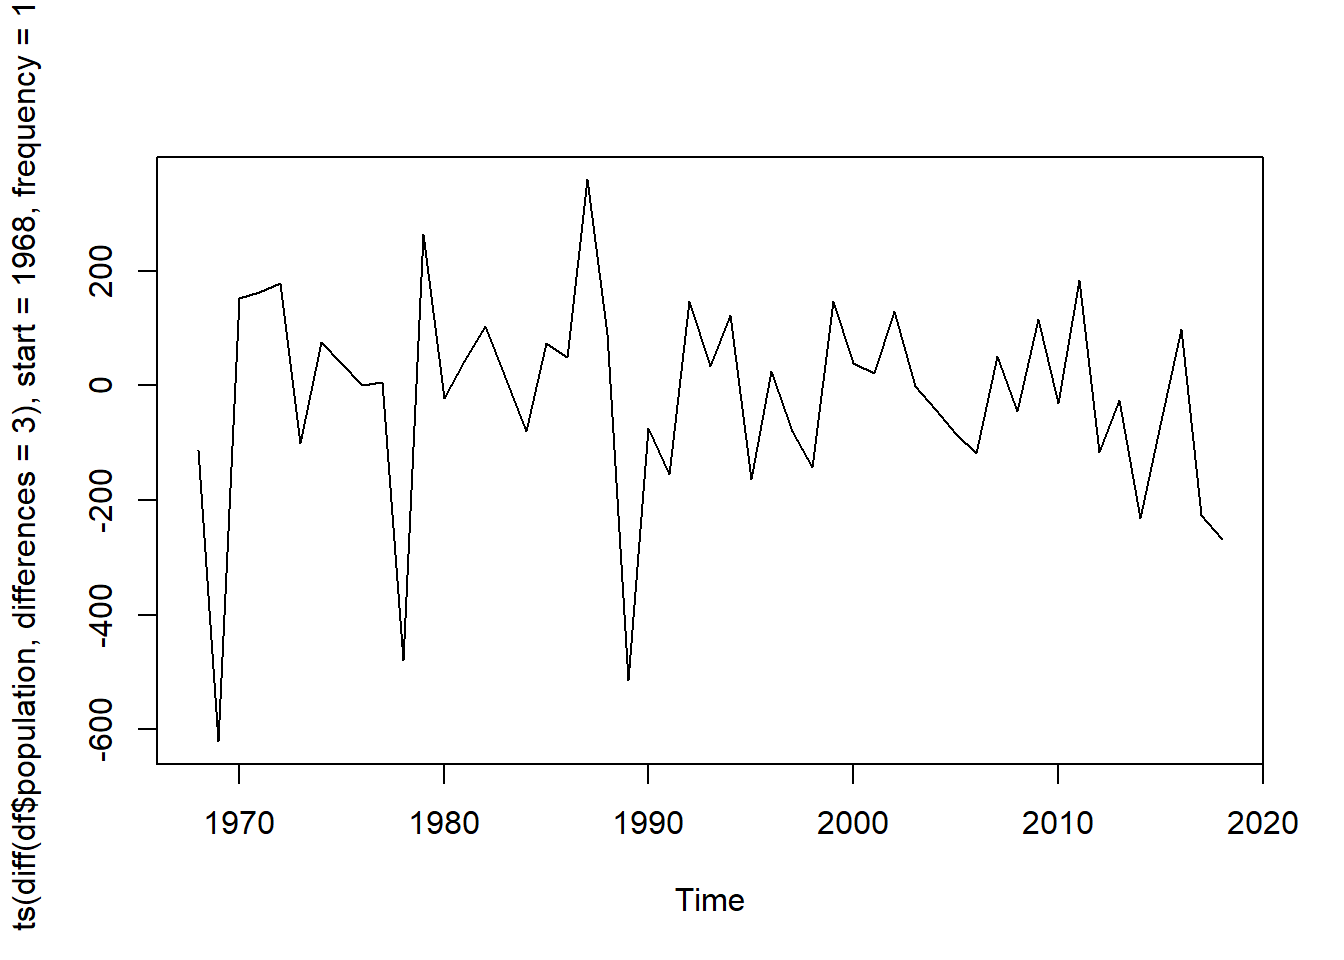
\includegraphics{davis_VAR_testing_files/figure-latex/unnamed-chunk-3-1.pdf}

\begin{Shaded}
\begin{Highlighting}[]
\CommentTok{\# {-}{-}{-}{-}{-}{-}{-} Cement {-}{-}{-}{-}{-}{-}{-}{-}{-}}

\FunctionTok{adf.test}\NormalTok{(df}\SpecialCharTok{$}\NormalTok{Cement)}\CommentTok{\# not stationary}
\end{Highlighting}
\end{Shaded}

\begin{verbatim}
## 
##  Augmented Dickey-Fuller Test
## 
## data:  df$Cement
## Dickey-Fuller = -2.4705, Lag order = 3, p-value = 0.385
## alternative hypothesis: stationary
\end{verbatim}

\begin{Shaded}
\begin{Highlighting}[]
\FunctionTok{adf.test}\NormalTok{(}\FunctionTok{diff}\NormalTok{(df}\SpecialCharTok{$}\NormalTok{Cement)) }\CommentTok{\#1st order dif {-}\textgreater{} becomes stationary}
\end{Highlighting}
\end{Shaded}

\begin{verbatim}
## 
##  Augmented Dickey-Fuller Test
## 
## data:  diff(df$Cement)
## Dickey-Fuller = -3.9342, Lag order = 3, p-value = 0.0191
## alternative hypothesis: stationary
\end{verbatim}

\begin{Shaded}
\begin{Highlighting}[]
\CommentTok{\# {-}{-}{-}{-}{-}{-}{-} housing {-}{-}{-}{-}{-}{-}{-}{-}{-}}

\FunctionTok{adf.test}\NormalTok{(df}\SpecialCharTok{$}\NormalTok{housing) }\CommentTok{\# not stationary}
\end{Highlighting}
\end{Shaded}

\begin{verbatim}
## 
##  Augmented Dickey-Fuller Test
## 
## data:  df$housing
## Dickey-Fuller = -2.3133, Lag order = 3, p-value = 0.4483
## alternative hypothesis: stationary
\end{verbatim}

\begin{Shaded}
\begin{Highlighting}[]
\FunctionTok{adf.test}\NormalTok{(}\FunctionTok{diff}\NormalTok{(df}\SpecialCharTok{$}\NormalTok{housing)) }\CommentTok{\#1st order dif {-}\textgreater{} becomes stationary}
\end{Highlighting}
\end{Shaded}

\begin{verbatim}
## Warning in adf.test(diff(df$housing)): p-value smaller than printed p-value
\end{verbatim}

\begin{verbatim}
## 
##  Augmented Dickey-Fuller Test
## 
## data:  diff(df$housing)
## Dickey-Fuller = -4.1928, Lag order = 3, p-value = 0.01
## alternative hypothesis: stationary
\end{verbatim}

\begin{Shaded}
\begin{Highlighting}[]
\CommentTok{\# {-}{-}{-}{-}{-}{-}{-} gasppi {-}{-}{-}{-}{-}{-}{-}{-}{-}}

\FunctionTok{adf.test}\NormalTok{(df}\SpecialCharTok{$}\NormalTok{gasppi) }\CommentTok{\# not stationary}
\end{Highlighting}
\end{Shaded}

\begin{verbatim}
## 
##  Augmented Dickey-Fuller Test
## 
## data:  df$gasppi
## Dickey-Fuller = -2.2159, Lag order = 3, p-value = 0.4876
## alternative hypothesis: stationary
\end{verbatim}

\begin{Shaded}
\begin{Highlighting}[]
\FunctionTok{adf.test}\NormalTok{(}\FunctionTok{diff}\NormalTok{(df}\SpecialCharTok{$}\NormalTok{gasppi,}\AttributeTok{differences =} \DecValTok{2}\NormalTok{)) }\CommentTok{\#2nd order dif {-}\textgreater{} becomes stationary}
\end{Highlighting}
\end{Shaded}

\begin{verbatim}
## Warning in adf.test(diff(df$gasppi, differences = 2)): p-value smaller than
## printed p-value
\end{verbatim}

\begin{verbatim}
## 
##  Augmented Dickey-Fuller Test
## 
## data:  diff(df$gasppi, differences = 2)
## Dickey-Fuller = -5.6787, Lag order = 3, p-value = 0.01
## alternative hypothesis: stationary
\end{verbatim}

\begin{Shaded}
\begin{Highlighting}[]
\CommentTok{\# {-}{-}{-}{-}{-}{-}{-} workers {-}{-}{-}{-}{-}{-}{-}{-}{-}}

\FunctionTok{adf.test}\NormalTok{(df}\SpecialCharTok{$}\NormalTok{workers) }\CommentTok{\# not stationary}
\end{Highlighting}
\end{Shaded}

\begin{verbatim}
## 
##  Augmented Dickey-Fuller Test
## 
## data:  df$workers
## Dickey-Fuller = -2.5487, Lag order = 3, p-value = 0.3535
## alternative hypothesis: stationary
\end{verbatim}

\begin{Shaded}
\begin{Highlighting}[]
\FunctionTok{adf.test}\NormalTok{(}\FunctionTok{diff}\NormalTok{(df}\SpecialCharTok{$}\NormalTok{workers)) }\CommentTok{\#2nd order dif {-}\textgreater{} becomes stationary}
\end{Highlighting}
\end{Shaded}

\begin{verbatim}
## 
##  Augmented Dickey-Fuller Test
## 
## data:  diff(df$workers)
## Dickey-Fuller = -3.6167, Lag order = 3, p-value = 0.04008
## alternative hypothesis: stationary
\end{verbatim}

\begin{Shaded}
\begin{Highlighting}[]
\CommentTok{\# {-}{-}{-}{-}{-}{-}{-} lime  {-}{-}{-}{-}{-}{-}{-}{-}{-}}

\FunctionTok{adf.test}\NormalTok{(df}\SpecialCharTok{$}\NormalTok{lime) }\CommentTok{\# not stationary}
\end{Highlighting}
\end{Shaded}

\begin{verbatim}
## 
##  Augmented Dickey-Fuller Test
## 
## data:  df$lime
## Dickey-Fuller = -1.8363, Lag order = 3, p-value = 0.6404
## alternative hypothesis: stationary
\end{verbatim}

\begin{Shaded}
\begin{Highlighting}[]
\FunctionTok{adf.test}\NormalTok{(}\FunctionTok{diff}\NormalTok{(df}\SpecialCharTok{$}\NormalTok{lime)) }\CommentTok{\#2nd order dif {-}\textgreater{} becomes stationary}
\end{Highlighting}
\end{Shaded}

\begin{verbatim}
## 
##  Augmented Dickey-Fuller Test
## 
## data:  diff(df$lime)
## Dickey-Fuller = -3.6948, Lag order = 3, p-value = 0.03356
## alternative hypothesis: stationary
\end{verbatim}

\begin{Shaded}
\begin{Highlighting}[]
\CommentTok{\# {-}{-}{-}{-}{-}{-}{-} silica {-}{-}{-}{-}{-}{-}{-}{-}{-}}

\FunctionTok{adf.test}\NormalTok{(df}\SpecialCharTok{$}\NormalTok{silica) }\CommentTok{\# not stationary}
\end{Highlighting}
\end{Shaded}

\begin{verbatim}
## 
##  Augmented Dickey-Fuller Test
## 
## data:  df$silica
## Dickey-Fuller = -2.2069, Lag order = 3, p-value = 0.4912
## alternative hypothesis: stationary
\end{verbatim}

\begin{Shaded}
\begin{Highlighting}[]
\FunctionTok{adf.test}\NormalTok{(}\FunctionTok{diff}\NormalTok{(df}\SpecialCharTok{$}\NormalTok{silica,}\AttributeTok{differences =} \DecValTok{2}\NormalTok{)) }\CommentTok{\#2nd order dif {-}\textgreater{} becomes stationary}
\end{Highlighting}
\end{Shaded}

\begin{verbatim}
## Warning in adf.test(diff(df$silica, differences = 2)): p-value smaller than
## printed p-value
\end{verbatim}

\begin{verbatim}
## 
##  Augmented Dickey-Fuller Test
## 
## data:  diff(df$silica, differences = 2)
## Dickey-Fuller = -4.7914, Lag order = 3, p-value = 0.01
## alternative hypothesis: stationary
\end{verbatim}

\hypertarget{testing-with-all-variables}{%
\subsection{Testing with all
variables}\label{testing-with-all-variables}}

\begin{Shaded}
\begin{Highlighting}[]
\CommentTok{\# {-}{-}{-}{-}{-}{-}{-}{-}{-} }\AlertTok{TESTING}\CommentTok{ WITH ALL VARIABLES {-}{-}{-}{-}{-}{-}{-}{-}{-}{-}{-}}

\NormalTok{diff\_1\_vars }\OtherTok{\textless{}{-}}\NormalTok{ df[,}\FunctionTok{c}\NormalTok{(}\StringTok{"cpi"}\NormalTok{,}\StringTok{"unemploy"}\NormalTok{,}\StringTok{"oilprice"}\NormalTok{,}\StringTok{"Cement"}\NormalTok{,}\StringTok{"housing"}\NormalTok{,}\StringTok{"workers"}\NormalTok{, }\StringTok{"gdp"}\NormalTok{,}\StringTok{"lime"}\NormalTok{)]}

\NormalTok{diff\_1\_vars }\OtherTok{\textless{}{-}} \FunctionTok{ts}\NormalTok{(diff\_1\_vars, }\AttributeTok{start =} \DecValTok{1968}\NormalTok{, }\AttributeTok{frequency =} \DecValTok{1}\NormalTok{)}
\NormalTok{diff\_1\_vars }\OtherTok{\textless{}{-}} \FunctionTok{lapply}\NormalTok{(diff\_1\_vars,}\ControlFlowTok{function}\NormalTok{(x) }\FunctionTok{diff}\NormalTok{(x)) }\CommentTok{\#reduced to 53 observations }

\NormalTok{diff\_2\_vars }\OtherTok{\textless{}{-}}\NormalTok{ df[,}\FunctionTok{c}\NormalTok{(}\StringTok{"silica"}\NormalTok{,}\StringTok{"gasppi"}\NormalTok{)]}
\NormalTok{diff\_2\_vars }\OtherTok{\textless{}{-}} \FunctionTok{ts}\NormalTok{(diff\_2\_vars, }\AttributeTok{start =} \DecValTok{1968}\NormalTok{, }\AttributeTok{frequency =} \DecValTok{1}\NormalTok{)}
\NormalTok{diff\_2\_vars }\OtherTok{\textless{}{-}} \FunctionTok{sapply}\NormalTok{(diff\_2\_vars, }\ControlFlowTok{function}\NormalTok{(x) }\FunctionTok{diff}\NormalTok{(x,}\AttributeTok{differences =} \DecValTok{2}\NormalTok{)) }\CommentTok{\#reduced to 52 observations }

\NormalTok{diff\_3\_vars }\OtherTok{\textless{}{-}} \FunctionTok{diff}\NormalTok{(}\FunctionTok{ts}\NormalTok{(df[,}\StringTok{"population"}\NormalTok{],}\AttributeTok{start =} \DecValTok{1968}\NormalTok{, }\AttributeTok{frequency =} \DecValTok{1}\NormalTok{),}\AttributeTok{differences =} \DecValTok{3}\NormalTok{) }\CommentTok{\#reduced to 51 observations }

\NormalTok{differenced\_df }\OtherTok{\textless{}{-}} \FunctionTok{cbind}\NormalTok{(}
  \FunctionTok{as.data.frame}\NormalTok{(diff\_1\_vars)[}\SpecialCharTok{{-}}\FunctionTok{c}\NormalTok{(}\DecValTok{1}\NormalTok{,}\DecValTok{2}\NormalTok{),],}
  \FunctionTok{as.data.frame}\NormalTok{(diff\_2\_vars)[}\SpecialCharTok{{-}}\DecValTok{1}\NormalTok{,],}
  \FunctionTok{as.data.frame}\NormalTok{(diff\_3\_vars)}
\NormalTok{)}

\CommentTok{\# turning it back into a time series format (this is in rates)}
\NormalTok{differenced\_df }\OtherTok{\textless{}{-}} \FunctionTok{ts}\NormalTok{(differenced\_df, }\AttributeTok{start =} \DecValTok{1971}\NormalTok{, }\AttributeTok{frequency =} \DecValTok{1}\NormalTok{)}


\DocumentationTok{\#\# {-}{-}{-} Affirming that all variables are now stationary {-}{-}{-}{-} POSITIVE}

\NormalTok{adf\_results }\OtherTok{\textless{}{-}} \FunctionTok{lapply}\NormalTok{(differenced\_df, }\ControlFlowTok{function}\NormalTok{(variable) \{}
\NormalTok{  adf\_result }\OtherTok{\textless{}{-}} \FunctionTok{adf.test}\NormalTok{(variable)}
  \FunctionTok{return}\NormalTok{(adf\_result)}
\NormalTok{\})}
\end{Highlighting}
\end{Shaded}

\begin{verbatim}
## Warning in adf.test(variable): p-value smaller than printed p-value

## Warning in adf.test(variable): p-value smaller than printed p-value

## Warning in adf.test(variable): p-value smaller than printed p-value

## Warning in adf.test(variable): p-value smaller than printed p-value

## Warning in adf.test(variable): p-value smaller than printed p-value
\end{verbatim}

\begin{Shaded}
\begin{Highlighting}[]
\ControlFlowTok{for}\NormalTok{ (i }\ControlFlowTok{in} \FunctionTok{seq\_along}\NormalTok{(adf\_results)) \{}
\NormalTok{  variable\_name }\OtherTok{\textless{}{-}} \FunctionTok{names}\NormalTok{(differenced\_df)[i]}
\NormalTok{  p\_value }\OtherTok{\textless{}{-}}\NormalTok{ adf\_results[[i]]}\SpecialCharTok{$}\NormalTok{p.value}
\NormalTok{  stationary\_status }\OtherTok{\textless{}{-}} \FunctionTok{ifelse}\NormalTok{(p\_value }\SpecialCharTok{\textless{}} \FloatTok{0.05}\NormalTok{, }\StringTok{"Stationary"}\NormalTok{, }\StringTok{"Non{-}Stationary"}\NormalTok{)}
  
  \FunctionTok{cat}\NormalTok{(}\StringTok{"Variable:"}\NormalTok{, variable\_name, }\StringTok{"}\SpecialCharTok{\textbackslash{}n}\StringTok{"}\NormalTok{)}
  \FunctionTok{cat}\NormalTok{(}\StringTok{"P{-}Value:"}\NormalTok{, p\_value, }\StringTok{"}\SpecialCharTok{\textbackslash{}n}\StringTok{"}\NormalTok{)}
  \FunctionTok{cat}\NormalTok{(}\StringTok{"Status:"}\NormalTok{, stationary\_status, }\StringTok{"}\SpecialCharTok{\textbackslash{}n\textbackslash{}n}\StringTok{"}\NormalTok{)}
\NormalTok{\}}
\end{Highlighting}
\end{Shaded}

\begin{verbatim}
## Variable: 
## P-Value: 0.01 
## Status: Stationary 
## 
## Variable: 
## P-Value: 0.01 
## Status: Stationary 
## 
## Variable: 
## P-Value: 0.03887001 
## Status: Stationary 
## 
## Variable: 
## P-Value: 0.0171151 
## Status: Stationary 
## 
## Variable: 
## P-Value: 0.02738807 
## Status: Stationary 
## 
## Variable: 
## P-Value: 0.04549926 
## Status: Stationary 
## 
## Variable: 
## P-Value: 0.03486656 
## Status: Stationary 
## 
## Variable: 
## P-Value: 0.03284613 
## Status: Stationary 
## 
## Variable: 
## P-Value: 0.01 
## Status: Stationary 
## 
## Variable: 
## P-Value: 0.01 
## Status: Stationary 
## 
## Variable: 
## P-Value: 0.01 
## Status: Stationary
\end{verbatim}

\hypertarget{var-stuff}{%
\subsection{VAR STUFF}\label{var-stuff}}

\begin{Shaded}
\begin{Highlighting}[]
\NormalTok{dummy\_var }\OtherTok{\textless{}{-}} \FunctionTok{data.frame}\NormalTok{(}\AttributeTok{year =} \DecValTok{1971}\SpecialCharTok{:}\DecValTok{2021}\NormalTok{) }\SpecialCharTok{|\textgreater{}}
  \FunctionTok{mutate}\NormalTok{(}\AttributeTok{value =} \FunctionTok{case\_when}\NormalTok{(year }\SpecialCharTok{\%in\%} \FunctionTok{c}\NormalTok{(}\DecValTok{2008}\NormalTok{,}\DecValTok{2009}\NormalTok{) }\SpecialCharTok{\textasciitilde{}} \DecValTok{1}\NormalTok{,}\ConstantTok{TRUE} \SpecialCharTok{\textasciitilde{}} \DecValTok{0}\NormalTok{))}

\NormalTok{dummy\_var }\OtherTok{\textless{}{-}} \FunctionTok{ts}\NormalTok{(dummy\_var[,}\SpecialCharTok{{-}}\DecValTok{1}\NormalTok{],}\AttributeTok{start =} \DecValTok{1971}\NormalTok{, }\AttributeTok{frequency =} \DecValTok{1}\NormalTok{)}
\NormalTok{merged\_data }\OtherTok{\textless{}{-}} \FunctionTok{cbind}\NormalTok{(differenced\_df,dummy\_var)}

\NormalTok{optimal\_lag }\OtherTok{\textless{}{-}} \FunctionTok{VARselect}\NormalTok{(merged\_data,}\AttributeTok{lag.max =} \DecValTok{10}\NormalTok{) }\CommentTok{\#gives AIC of 5, which is interesting...}
\NormalTok{optimal\_lag }\OtherTok{\textless{}{-}}\NormalTok{ optimal\_lag}\SpecialCharTok{$}\NormalTok{selection[}\DecValTok{1}\NormalTok{]}
\NormalTok{var\_model }\OtherTok{\textless{}{-}} \FunctionTok{VAR}\NormalTok{(merged\_data, }\AttributeTok{p =} \DecValTok{1}\NormalTok{, }\AttributeTok{type =} \StringTok{"none"}\NormalTok{) }\CommentTok{\#I used a manual lag of 1}

\NormalTok{years\_ahead }\OtherTok{\textless{}{-}} \DecValTok{29} \CommentTok{\#number of years to get to 2050}
\NormalTok{forecast }\OtherTok{\textless{}{-}} \FunctionTok{predict}\NormalTok{(var\_model, }\AttributeTok{n.ahead =}\NormalTok{ years\_ahead)}
\FunctionTok{par}\NormalTok{(}\AttributeTok{mar =} \FunctionTok{c}\NormalTok{(}\DecValTok{1}\NormalTok{, }\DecValTok{1}\NormalTok{, }\DecValTok{1}\NormalTok{, }\DecValTok{1}\NormalTok{))}
\FunctionTok{plot}\NormalTok{(forecast)}
\end{Highlighting}
\end{Shaded}

\includegraphics{davis_VAR_testing_files/figure-latex/unnamed-chunk-5-1.pdf}

\hypertarget{plotting-results}{%
\subsection{Plotting Results}\label{plotting-results}}

\begin{Shaded}
\begin{Highlighting}[]
\NormalTok{forecast\_original }\OtherTok{\textless{}{-}} \FunctionTok{cumsum}\NormalTok{(forecast}\SpecialCharTok{$}\NormalTok{fcst}\SpecialCharTok{$}\NormalTok{differenced\_df.Cement[,}\DecValTok{1}\NormalTok{]) }\SpecialCharTok{+}\NormalTok{ df}\SpecialCharTok{$}\NormalTok{Cement[}\FunctionTok{length}\NormalTok{(df}\SpecialCharTok{$}\NormalTok{Cement)]}\CommentTok{\#the original value in 1968}

\NormalTok{df1 }\OtherTok{\textless{}{-}} \FunctionTok{data.frame}\NormalTok{(df}\SpecialCharTok{$}\NormalTok{Cement)}
\FunctionTok{colnames}\NormalTok{(df1) }\OtherTok{\textless{}{-}} \StringTok{"cement"}
\NormalTok{df2 }\OtherTok{\textless{}{-}} \FunctionTok{data.frame}\NormalTok{(forecast\_original)}
\FunctionTok{colnames}\NormalTok{(df2) }\OtherTok{\textless{}{-}} \StringTok{"cement"}

\NormalTok{merged\_temp }\OtherTok{\textless{}{-}} \FunctionTok{rbind}\NormalTok{(df1, df2)}
\NormalTok{years\_temp }\OtherTok{\textless{}{-}} \FunctionTok{data.frame}\NormalTok{(}\DecValTok{1968}\SpecialCharTok{:}\NormalTok{(}\DecValTok{2021}\SpecialCharTok{+}\NormalTok{years\_ahead))}
\FunctionTok{colnames}\NormalTok{(years\_temp) }\OtherTok{\textless{}{-}} \StringTok{"years"}

\NormalTok{plot\_final }\OtherTok{\textless{}{-}} \FunctionTok{cbind}\NormalTok{(years\_temp,merged\_temp)}

\NormalTok{plot\_final }\SpecialCharTok{|\textgreater{}}
  \FunctionTok{ggplot}\NormalTok{(}\FunctionTok{aes}\NormalTok{(}\AttributeTok{x =}\NormalTok{ years, }\AttributeTok{y =}\NormalTok{ cement)) }\SpecialCharTok{+} 
  \FunctionTok{geom\_line}\NormalTok{() }\SpecialCharTok{+} 
  \FunctionTok{xlab}\NormalTok{(}\StringTok{"Years"}\NormalTok{) }\SpecialCharTok{+} \FunctionTok{ylab}\NormalTok{(}\StringTok{"Cement (million metric tons)"}\NormalTok{) }\SpecialCharTok{+}
  \FunctionTok{scale\_y\_continuous}\NormalTok{(}\AttributeTok{labels =}\NormalTok{ scales}\SpecialCharTok{::}\FunctionTok{comma\_format}\NormalTok{(}\AttributeTok{scale =} \FloatTok{1e{-}3}\NormalTok{)) }\SpecialCharTok{+} 
  \FunctionTok{scale\_x\_continuous}\NormalTok{(}\AttributeTok{breaks =} \FunctionTok{seq}\NormalTok{(}\DecValTok{1970}\NormalTok{, }\DecValTok{2050}\NormalTok{, }\AttributeTok{by =} \DecValTok{5}\NormalTok{)) }\SpecialCharTok{+}
  \FunctionTok{geom\_vline}\NormalTok{(}\AttributeTok{xintercept =} \DecValTok{2021}\NormalTok{, }\AttributeTok{color =} \StringTok{"red"}\NormalTok{, }\AttributeTok{linetype =} \StringTok{"dashed"}\NormalTok{)}
\end{Highlighting}
\end{Shaded}

\includegraphics{davis_VAR_testing_files/figure-latex/unnamed-chunk-6-1.pdf}

\hypertarget{testing-with-limited-variables-filtered-based-on-correlation-distribution-matrix-to-prevent-cross-validation}{%
\subsection{Testing with limited variables filtered based on correlation
distribution matrix (to prevent
cross-validation)}\label{testing-with-limited-variables-filtered-based-on-correlation-distribution-matrix-to-prevent-cross-validation}}

Variables considered: cpi, gdp, Cement (dependent var), housing, lime,
gasppi

outta here: oilprice, population, workers, silica

\begin{Shaded}
\begin{Highlighting}[]
\CommentTok{\# {-}{-}{-}{-}{-}{-}{-}{-}{-} }\AlertTok{TESTING}\CommentTok{ WITH LIMITED VARIABLES {-}{-}{-}{-}{-}{-}{-}{-}{-}{-}{-} cpi, housing, gdp , Cement, oilprice, gasppi}


\NormalTok{df}\SpecialCharTok{$}\NormalTok{gdp }\OtherTok{\textless{}{-}}\NormalTok{ df}\SpecialCharTok{$}\NormalTok{gdp}\SpecialCharTok{/}\DecValTok{1000000000}

\NormalTok{diff\_1\_vars\_lim }\OtherTok{\textless{}{-}}\NormalTok{ df[,}\FunctionTok{c}\NormalTok{(}\StringTok{"cpi"}\NormalTok{,}\StringTok{"Cement"}\NormalTok{,}\StringTok{"housing"}\NormalTok{,}\StringTok{"gdp"}\NormalTok{,}\StringTok{"lime"}\NormalTok{)]}
\NormalTok{diff\_1\_vars\_lim }\OtherTok{\textless{}{-}} \FunctionTok{ts}\NormalTok{(diff\_1\_vars\_lim, }\AttributeTok{start =} \DecValTok{1968}\NormalTok{, }\AttributeTok{frequency =} \DecValTok{1}\NormalTok{)}
\NormalTok{diff\_1\_vars\_lim }\OtherTok{\textless{}{-}} \FunctionTok{lapply}\NormalTok{(diff\_1\_vars\_lim,}\ControlFlowTok{function}\NormalTok{(x) }\FunctionTok{diff}\NormalTok{(x))}
\NormalTok{diff\_2\_vars\_lim }\OtherTok{\textless{}{-}} \FunctionTok{diff}\NormalTok{(}\FunctionTok{ts}\NormalTok{(df[,}\StringTok{"gasppi"}\NormalTok{], }\AttributeTok{start =} \DecValTok{1968}\NormalTok{, }\AttributeTok{frequency =} \DecValTok{1}\NormalTok{),}\AttributeTok{differences =} \DecValTok{2}\NormalTok{)}

\NormalTok{dummy\_var }\OtherTok{\textless{}{-}} \FunctionTok{data.frame}\NormalTok{(}\AttributeTok{year =} \DecValTok{1970}\SpecialCharTok{:}\DecValTok{2021}\NormalTok{) }\SpecialCharTok{|\textgreater{}}
  \FunctionTok{mutate}\NormalTok{(}\AttributeTok{value =} \FunctionTok{case\_when}\NormalTok{(year }\SpecialCharTok{\%in\%} \FunctionTok{c}\NormalTok{(}\DecValTok{1973}\NormalTok{, }\DecValTok{1974}\NormalTok{,}\DecValTok{1979}\NormalTok{,}\DecValTok{2008}\NormalTok{) }\SpecialCharTok{\textasciitilde{}} \DecValTok{1}\NormalTok{,}\ConstantTok{TRUE} \SpecialCharTok{\textasciitilde{}} \DecValTok{0}\NormalTok{)) }\CommentTok{\#includes 1973, 1974, and 1979, and 1980}


\NormalTok{differenced\_df\_lim }\OtherTok{\textless{}{-}} \FunctionTok{cbind}\NormalTok{(}
  \FunctionTok{as.data.frame}\NormalTok{(}\FunctionTok{lapply}\NormalTok{(diff\_1\_vars\_lim, }\ControlFlowTok{function}\NormalTok{(x) }\FunctionTok{window}\NormalTok{(x, }\AttributeTok{start =} \DecValTok{1970}\NormalTok{))), }
  \FunctionTok{as.data.frame}\NormalTok{(}\FunctionTok{lapply}\NormalTok{(diff\_2\_vars\_lim, }\ControlFlowTok{function}\NormalTok{(x) }\FunctionTok{window}\NormalTok{(x, }\AttributeTok{start =} \DecValTok{1970}\NormalTok{)))}
  
\NormalTok{)}

\NormalTok{differenced\_df\_lim }\OtherTok{\textless{}{-}} \FunctionTok{ts}\NormalTok{(differenced\_df\_lim, }\AttributeTok{start =} \DecValTok{1970}\NormalTok{, }\AttributeTok{frequency =} \DecValTok{1}\NormalTok{)}

\NormalTok{optimal\_lag\_lim }\OtherTok{\textless{}{-}} \FunctionTok{VARselect}\NormalTok{(differenced\_df\_lim,}\AttributeTok{lag.max =} \DecValTok{7}\NormalTok{) }\CommentTok{\#gives AIC of 5, which is interesting...}
\CommentTok{\# optimal\_lag\_lim \textless{}{-} optimal\_lag$selection[1]}
\NormalTok{var\_model\_lim }\OtherTok{\textless{}{-}} \FunctionTok{VAR}\NormalTok{(differenced\_df\_lim, }\AttributeTok{p =} \DecValTok{1}\NormalTok{, }\AttributeTok{type =} \StringTok{"const"}\NormalTok{)}

\NormalTok{forecast\_lim }\OtherTok{\textless{}{-}} \FunctionTok{predict}\NormalTok{(var\_model\_lim, }\AttributeTok{n.ahead =} \DecValTok{29}\NormalTok{)}
\FunctionTok{par}\NormalTok{(}\AttributeTok{mar =} \FunctionTok{c}\NormalTok{(}\DecValTok{1}\NormalTok{, }\DecValTok{1}\NormalTok{, }\DecValTok{1}\NormalTok{, }\DecValTok{1}\NormalTok{))}
\FunctionTok{plot}\NormalTok{(forecast\_lim)}
\end{Highlighting}
\end{Shaded}

\includegraphics{davis_VAR_testing_files/figure-latex/unnamed-chunk-7-1.pdf}

\begin{Shaded}
\begin{Highlighting}[]
\NormalTok{forecast\_original\_lim }\OtherTok{\textless{}{-}} \FunctionTok{cumsum}\NormalTok{(forecast\_lim}\SpecialCharTok{$}\NormalTok{fcst}\SpecialCharTok{$}\NormalTok{Cement[,}\DecValTok{1}\NormalTok{]) }\SpecialCharTok{+}\NormalTok{ df}\SpecialCharTok{$}\NormalTok{Cement[}\FunctionTok{length}\NormalTok{(df}\SpecialCharTok{$}\NormalTok{Cement)]}\CommentTok{\#the original value in 2021}
\CommentTok{\# forecast\_original\_lim\_lower\_upper \textless{}{-}apply(forecast\_lim$fcst$Cement[,2:3],2,cumsum) + df$Cement[length(df$Cement)]}

\NormalTok{df1 }\OtherTok{\textless{}{-}} \FunctionTok{data.frame}\NormalTok{(df}\SpecialCharTok{$}\NormalTok{Cement)}
\FunctionTok{colnames}\NormalTok{(df1) }\OtherTok{\textless{}{-}} \StringTok{"cement"}
\NormalTok{df2 }\OtherTok{\textless{}{-}} \FunctionTok{data.frame}\NormalTok{(forecast\_original\_lim)}
\FunctionTok{colnames}\NormalTok{(df2) }\OtherTok{\textless{}{-}} \StringTok{"cement"}

\NormalTok{merged\_df\_lim }\OtherTok{\textless{}{-}} \FunctionTok{rbind}\NormalTok{(df1, df2)}
\NormalTok{years\_lim }\OtherTok{\textless{}{-}} \FunctionTok{data.frame}\NormalTok{(}\DecValTok{1968}\SpecialCharTok{:}\DecValTok{2050}\NormalTok{)}
\FunctionTok{colnames}\NormalTok{(years\_lim) }\OtherTok{\textless{}{-}} \StringTok{"years"}

\NormalTok{plot\_lim }\OtherTok{\textless{}{-}} \FunctionTok{cbind}\NormalTok{(years\_lim,merged\_df\_lim)}

\NormalTok{plot\_lim }\SpecialCharTok{|\textgreater{}}
  \FunctionTok{ggplot}\NormalTok{(}\FunctionTok{aes}\NormalTok{(}\AttributeTok{x =}\NormalTok{ years, }\AttributeTok{y =}\NormalTok{ cement)) }\SpecialCharTok{+} 
  \FunctionTok{geom\_line}\NormalTok{() }\SpecialCharTok{+} 
  \FunctionTok{xlab}\NormalTok{(}\StringTok{"Years"}\NormalTok{) }\SpecialCharTok{+} \FunctionTok{ylab}\NormalTok{(}\StringTok{"Cement (million metric tons)"}\NormalTok{) }\SpecialCharTok{+}
  \FunctionTok{scale\_y\_continuous}\NormalTok{(}\AttributeTok{labels =}\NormalTok{ scales}\SpecialCharTok{::}\FunctionTok{comma\_format}\NormalTok{(}\AttributeTok{scale =} \FloatTok{1e{-}3}\NormalTok{)) }\SpecialCharTok{+}
  \FunctionTok{scale\_x\_continuous}\NormalTok{(}\AttributeTok{breaks =} \FunctionTok{seq}\NormalTok{(}\DecValTok{1970}\NormalTok{, }\DecValTok{2050}\NormalTok{, }\AttributeTok{by =} \DecValTok{5}\NormalTok{)) }\SpecialCharTok{+}
  \FunctionTok{geom\_vline}\NormalTok{(}\AttributeTok{xintercept =} \DecValTok{2021}\NormalTok{, }\AttributeTok{color =} \StringTok{"red"}\NormalTok{, }\AttributeTok{linetype =} \StringTok{"dashed"}\NormalTok{)}
\end{Highlighting}
\end{Shaded}

\includegraphics{davis_VAR_testing_files/figure-latex/unnamed-chunk-7-2.pdf}

\hypertarget{model-diagnosis-for-limited-variables-one-not-final-yet}{%
\subsection{Model Diagnosis for limited variables one (NOT FINAL
YET)}\label{model-diagnosis-for-limited-variables-one-not-final-yet}}

\begin{Shaded}
\begin{Highlighting}[]
\CommentTok{\# Residual Analysis}
\NormalTok{serial\_test }\OtherTok{\textless{}{-}} \FunctionTok{serial.test}\NormalTok{(var\_model\_lim, }\AttributeTok{lags.pt =} \DecValTok{1}\NormalTok{) }\CommentTok{\#passes this test because p{-}value \textgreater{} 0.05 (yes i meant to type greater)}

\CommentTok{\# Normality Test}
\NormalTok{residuals }\OtherTok{\textless{}{-}} \FunctionTok{resid}\NormalTok{(var\_model\_lim)}

\FunctionTok{par}\NormalTok{( }\AttributeTok{mfrow=} \FunctionTok{c}\NormalTok{(}\DecValTok{3}\NormalTok{,}\DecValTok{2}\NormalTok{) )}
\NormalTok{resdulpdf}\OtherTok{\textless{}{-}}\FunctionTok{density}\NormalTok{(residuals[,}\StringTok{"cpi"}\NormalTok{])}
\FunctionTok{plot}\NormalTok{(resdulpdf,}\AttributeTok{main=}\StringTok{\textquotesingle{}CPI Residual shape Plot\textquotesingle{}}\NormalTok{,}\AttributeTok{xlab=}\StringTok{\textquotesingle{}CPI Residuals\textquotesingle{}}\NormalTok{)}
\NormalTok{resdulpdf}\OtherTok{\textless{}{-}}\FunctionTok{density}\NormalTok{(residuals[,}\StringTok{"gdp"}\NormalTok{])}
\FunctionTok{plot}\NormalTok{(resdulpdf,}\AttributeTok{main=}\StringTok{\textquotesingle{}GDP Residual shape Plot\textquotesingle{}}\NormalTok{,}\AttributeTok{xlab=}\StringTok{\textquotesingle{}GDP Residuals\textquotesingle{}}\NormalTok{)}
\NormalTok{resdulpdf}\OtherTok{\textless{}{-}}\FunctionTok{density}\NormalTok{(residuals[,}\StringTok{"Cement"}\NormalTok{])}
\FunctionTok{plot}\NormalTok{(resdulpdf,}\AttributeTok{main=}\StringTok{\textquotesingle{}Cement Residual shape Plot\textquotesingle{}}\NormalTok{,}\AttributeTok{xlab=}\StringTok{\textquotesingle{}Cement Residuals\textquotesingle{}}\NormalTok{)}
\NormalTok{resdulpdf}\OtherTok{\textless{}{-}}\FunctionTok{density}\NormalTok{(residuals[,}\StringTok{"housing"}\NormalTok{])}
\FunctionTok{plot}\NormalTok{(resdulpdf,}\AttributeTok{main=}\StringTok{\textquotesingle{}Housing Residual shape Plot\textquotesingle{}}\NormalTok{,}\AttributeTok{xlab=}\StringTok{\textquotesingle{}HOusing Residuals\textquotesingle{}}\NormalTok{)}
\NormalTok{resdulpdf}\OtherTok{\textless{}{-}}\FunctionTok{density}\NormalTok{(residuals[,}\StringTok{"gasppi"}\NormalTok{])}
\FunctionTok{plot}\NormalTok{(resdulpdf,}\AttributeTok{main=}\StringTok{\textquotesingle{}gasppi Residual shape Plot\textquotesingle{}}\NormalTok{,}\AttributeTok{xlab=}\StringTok{\textquotesingle{}gasppi Residuals\textquotesingle{}}\NormalTok{)}
\NormalTok{resdulpdf}\OtherTok{\textless{}{-}}\FunctionTok{density}\NormalTok{(residuals[,}\StringTok{"lime"}\NormalTok{])}
\FunctionTok{plot}\NormalTok{(resdulpdf,}\AttributeTok{main=}\StringTok{\textquotesingle{}lime Residual shape Plot\textquotesingle{}}\NormalTok{,}\AttributeTok{xlab=}\StringTok{\textquotesingle{}lime Residuals\textquotesingle{}}\NormalTok{)}
\end{Highlighting}
\end{Shaded}

\includegraphics{davis_VAR_testing_files/figure-latex/unnamed-chunk-8-1.pdf}

\begin{Shaded}
\begin{Highlighting}[]
\NormalTok{arch\_test }\OtherTok{\textless{}{-}} \FunctionTok{arch.test}\NormalTok{(var\_model\_lim)}
\end{Highlighting}
\end{Shaded}


\end{document}
